%!TEX root = ../../proposal.tex

\section*{Abstract}

% Write a brief summary of the proposal. The summary should not exceed 120 words and best be a paragraph long. The summary should include a few lines about the background information, the main research question or problem that you want to write about, and your research methods. The proposal summary should not contain any references or citations. Remember that your entire proposal cannot exceed 1500 words, so choose the words in this section carefully. The 1500 words you will write in the proposal document will exclude any words contained in the tables, figures, and references. You can use this template for writing your proposal. 


%10-20 pages maximum

%Abstract
%Table of contents
%Introduction
%Background
%Goal and Objectives
%Methodology
%Timeplan
%Discussion/Conclusion
%Acknowledgements
%References
%Appendix

\tableofcontents

\clearpage

\section{Introduction}

Over the last decades many researchers studied the stock market and tried to analyze and build a model for stock price prediction.
Several of them followed the efficient market hypothesis \cite{Basu1977,Fama1995,Malkiel2003} which states that the stock market fully reflects all available information.
Due to this assumption price changes can be just be triggered by new or changed information.
Because news are not predictable and occur randomly stock prices should also follow a random walk pattern.
The best bet for the next price would be the current price of the share. 
Other studies tried to create a prediction model for share prices based on historical data \cite{Nguyen2015a}.

In the last years keywords like artificial intelligence, option mining and sentiment analysis arose.
So researchers used these technologies to enhance their prediction models.
They tried to incorporate the public mood and apply it to prediction models of share indices such as \cite{Bollen2011a,Mittal2012a,Nguyen2015a,Pagolu2016a,Zhang2011a} or politics as \cite{Oconnor2010a,Patodkar2016a}.
The source of analyzed data has been news for a long time and in recent times social media.
Social media is very interesting due the fact that many people are stating their opinion unfiltered publicly.
Twitter is a well known social media where users can post their opinions publicly and categorize them using hashtags.

\section{Background} 
\label{s:background}

This section should provide the theoretical background and the foundation of the conducted study.
Therefore, this section is structured as follows: 
first, an introduction into option mining will be given in \autoref{ss:background-optionmining};
second, the market of social networks will be examined in \autoref{ss:background-socialnetworks};
and third, related work of stock market prediction will be presented in \autoref{ss:background-stockmarketprediction}.

\subsection{Option Mining} 
\label{ss:background-optionmining}

Option mining is defined as extracting opinions from unstructured data using natural language processing techniques \cite[page 411]{Liu2007}.

According to Pang and Lee the two terms \emph{option mining} and \emph{sentiment analysis} are mere synonyms within this field of study \cite{Pang2008c}.
Therefore, this study will use the terms interchangeably.

There are several types of option mining available:

\begin{enumerate}
	\item 
	Sentiment classification: 
	This task is performed on a document level and classifies the text as positive or negative. 
	No further analysis is made what people may like or dislike 
	\cite[page 411]{Liu2007}.
	
	\item 
	Feature-based opinion mining and summarization: 
	This task dives deep into the text and analyzes the sentences on it's own.
	Furthermore, it discovers the opinions on objects which are liked or disliked.
	An object may be a product, service, topic or organization. 
	For example in an product review it detects the product features which have been described 
	\cite[page 412]{Liu2007}.
	
	\item
	Comparative sentence and relation mining:
	In this type of task product features are compared to the same or similar feature of another product.
	For example comparing two cameras: "the battery life of camera A is much shorter than that of camera B" 
	\cite[page 412]{Liu2007}. 
\end{enumerate}

This study will focus on short documents with given keywords in it. 
Therefore, we assume that the documents describing our targeted topic.
As a result the study will focus on sentiment classification.

Sentiment classification has some similarities with topic-based text classification, which classifies the topic of documents into predefined topic classes, for example sports, science or politics.
In topic based classification topic words are important, while they are unimportant for sentiment classification \cite[page 412f]{Liu2007}.

\subsubsection{Algorithms}
\label{sss:background-optionmining-alogrithms}

\citeauthor{Pang2002} performed a study which analyzed several machine learning algorithms and their suitability with sentiment classification.
These three algorithms have shown a good performance in text categorization studies and therefore they tried to apply these algorithms to sentiment classification \cite{Pang2002}.

\begin{table}
	\begin{center}
		\begin{tabular}{l l}
			\textbf{Element} & \textbf{Description} \\ \hline
			$c$ & Spefific document class \\
			$C$ & Document classes \\
			$d$ & Specific document \\
			$D$ & Documents \\
			$f_i$ & Specific feature \\
			$m$ & Count of features \\
			$n_i(d)$ & Count of features $i$ in document $d$ \\
			$P(x)$ & Probability of x \\
		\end{tabular}
	
		\label{tab:background-optionmining-algorithms-variables}
		\caption{Used variables by the algorithms}		
	\end{center}
\end{table}

\begin{description}
	\item[Naive Bayes.] 
	The Naive Bayes (NB) algorithm calculates the probabilities that a document $d$ belong to a class $c$.
	Furthermore, it implies that all classes are independent to each other, which does not hold true very often in a real world scenario.
	In sentiment classification tasks there are two classes available: positive and negative.
	Therefore the text is classified as class $c$ where $c* = arg max_c P(c | d)$.
	The general Bayes classifier can be seen in \autoref{eq:background-optionmining-algorithms-bayes} \cite{Pang2002}.
	
	\begin{equation}
		P_{NB}(c|d) = \frac{P(c) (\prod_{i=1}^{m} P(f_i|c)^{n_i(d)}) }{P(d)}
		\label{eq:background-optionmining-algorithms-bayes}
	\end{equation}
	
	Despite the fact that the Naive Bayes algorithm is very simple and the assumption of independent classes does not hold true in a real world scenario it performs surprisingly well \cite{Pang2002}.
	
	\item[Maximum Entropy Classification.]
  The Maximum Entropy Classification (MaxEnt for short) succeeded in a number of language processing applications.
  The exponential form of the Maximum Entropy Classifier can be seen in \autoref{eq:background-optionmining-algorithms-maximumentropy} \cite{Pang2002}.
  
  \begin{equation}
		P_{ME}(c|d) = \frac{1}{Z(d)} exp \left( \sum_i^m \lambda_{i,c}F_{i,c}(d,c) \right)
		\label{eq:background-optionmining-algorithms-maximumentropy}
  \end{equation}
  
  Whereas $Z(d)$ is a normalization function as depicted in \autoref{eq:background-optionmining-algorithms-maximumentropy_Zd} \cite{Nigam1999} and $F_{i,c}(d,c)$ is a feature/class function for feature $f_i$ and class $c$ which is defined in \autoref{eq:background-optionmining-algorithms-maximumentropy_fic}.

  \begin{equation}
    Z(d) = \sum_c exp(\sum_i \lambda_{i,c} F_{i,c}(d,c))
      \label{eq:background-optionmining-algorithms-maximumentropy_Zd}
  \end{equation}

  \begin{equation}
  F_{i,c}(d,c') = 
    \begin{cases}
      1, & n_i(d) > 0 \text{ and } c' = c \\
      0  & \text{otherwise}
    \end{cases}
		\label{eq:background-optionmining-algorithms-maximumentropy_fic}
  \end{equation}

  $\lambda_{i,c}$ are feature weight parameters. A larger value of that parameter means that feature $f_i$ is considered as strong indicator for class $c$.
  The values for $\lambda_{i,c}$ are set in a way that the entropy of the training data set is maximized \cite{Pang2002}.
  	
	\item[Support Vector Machine.]
   Support Vector Machines are large-margin classifiers in contrast to the probabilistic Naive Bayes and Maximum Entropy.
   That means that in the two-category case (positive or negative) the training procedure looking for a hyperplane which maximizes the margin between the two groups \cite{Pang2002}.
   This scenario is depicted in \autoref{fig:background-optionmining-algorithms-svm} \cite[p. 275]{Cortes1995}.
      
   \begin{figure}[ht]
    \centering
    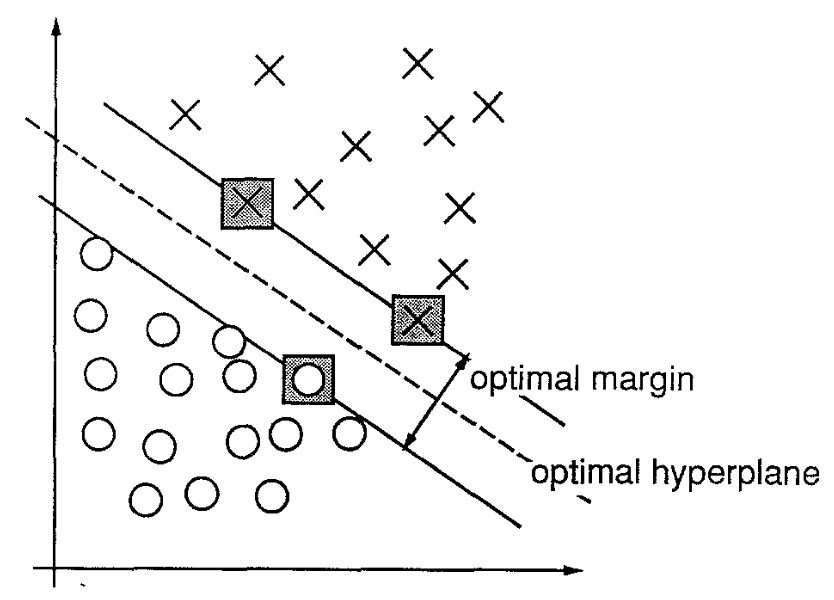
\includegraphics[width=.7\textwidth]{images/svm.png}
    \caption{An example of a two-category case, from \cite[p. 275]{Cortes1995}}
    \label{fig:background-optionmining-algorithms-svm}
  \end{figure}
	
\end{description}

%algorithms
%SVM
%naive bayesian

%bag of words 
%unigrams
%bigrams
%trigrams

%pre processing
%stop word
%stemming

\subsection{Social networks/microblogging services}
\label{ss:background-socialnetworks}

In the last years many social networks started and many of them disappeared again.
There are several types of social networks available today: some of them are built on videos others on pictures and some of them mostly on text.
Those which are built on text are more easy to analyze and searchable for researchers worldwide.
But there are some constants in this field: Twitter, to identify one of them.
Twitter has become a valueable source of opinions, data and information for various researches \cite{Barbosa2010}.

Messages on Twitter are called tweets and are limited in length (140 for tweets before November 7th 2017; 280 characters since then, at least for english tweets \cite{Rosen2017TweetingEasier}) users have to concentrate on a specific topic precisely.
Therefore, Twitter is the perfect source of the public opinion as users discussing anything on Twitter \cite{Pagolu2016a}.

As a result the fields in which researches have used data from Twitter ranging from public opinions for politicans and polls (see \cite{Oconnor2010a,Patodkar2016a}) to the stock market and the prediction of stock prices and other factors (see \cite{Bollen2011a,Mittal2012a,Nguyen2015a,Pagolu2016a,Zhang2011a}).

% On the other hand keywords like cloud, machine learning and artificial intelligence are everywhere. 
% Amazon, Facebook, Google, IBM and Microsoft and other big players of the industry are making massive progress in these fields.

\subsection{Stock Market Prediction} 
\label{ss:background-stockmarketprediction}

\citeauthor{Bollen2011a} noted that many researches assumed that the stock market is based on the random walk theory and the Efficient Market Hypothesis (EMH).
The EMH assumes that stock market prices are driven by new information such as news and will less depend on the current price or historical prices.
As news are unpredictable the stock market prices will follow a random walk pattern \cite{Bollen2011a}.

But \citeauthor{Bollen2011a} stated also that stock prices aren't following the random walk pattern completely and can therefore predicted in some way.
They stated that information available online may act as early indicators for changes.
This include the Google search queries which provide an early indicator for disease infections (see \url{https://www.google.org/flutrends/}) \cite{Bollen2011a}.

\section{Goal and Objectives}

The goal of this research to analyze the correlation between sentiment of tweets and share movement of automotive companies.
This goal will be met by achieving the following objectives:

\begin{itemize}
	\item Determine companies, keywords and stock symbols to analyze
	\item Gather tweets and stock prices
  \item Normalization of tweets
  \item Determine sentiment of tweets
  \item Comparing sentiment time series with share prices
\end{itemize}

\section{Population and Methods}

\subsection{Determine companies, keywords and stock symbols to analyze}

First, a list of automotive companies is needed.
These companies must be traded on a stock exchange to perform the comparison with tweet sentiments.
As a single company may own several car brands a list of all brands has been set up.
The result of the analysis is depicted in \autoref{tab:brands}.
Both brands which aren't customer facing passenger car brands and brands which do not longer exist have been omitted.
Furthermore, the brands have been grouped by their owning company.

  \begin{longtable}[c]{ll}
   \bfseries{Car brand} & \bfseries{Owning Company}  \\ \hline
  \endfirsthead
  %
  \multicolumn{2}{c}%
  {{\bfseries Table \thetable\ continued from previous page}} \\
   &  \\
  \endhead
  %
  BMW  & BMW \cite[p.30]{BMWGroup2017} \\
  Mini  & BMW  \cite[p.30]{BMWGroup2017} \\
  Rolls-Royce   & BMW \cite[p.30]{BMWGroup2017} \\
  Mercedes-AMG & Daimler \cite[p.90]{DaimlerAG2018} \\
  Mercedes-Benz  & Daimler \cite[p.90]{DaimlerAG2018} \\
  Mercedes-Maybach & Daimler \cite[p.90]{DaimlerAG2018} \\
  Smart  & Daimler \cite[p.90]{DaimlerAG2018} \\
  Alfa Romeo & Fiat Chrysler Automobiles \cite[p.32]{FiatChryslerAutomobiles2018a} \\
  Chrysler & Fiat Chrysler Automobiles \cite[p.32]{FiatChryslerAutomobiles2018a} \\
  Dodge & Fiat Chrysler Automobiles \cite[p.32]{FiatChryslerAutomobiles2018a} \\
  Fiat & Fiat Chrysler Automobiles \cite[p.32]{FiatChryslerAutomobiles2018a} \\
  Fiat Professional & Fiat Chrysler Automobiles \cite[p.32]{FiatChryslerAutomobiles2018a} \\
  Jeep & Fiat Chrysler Automobiles \cite[p.32]{FiatChryslerAutomobiles2018a} \\
  Lancia & Fiat Chrysler Automobiles \cite[p.32]{FiatChryslerAutomobiles2018a} \\
  RAM & Fiat Chrysler Automobiles \cite[p.32]{FiatChryslerAutomobiles2018a} \\
  Ford & Ford Motor Company \cite[p.18]{FordMotorCompany2018} \\
  Lincoln  & Ford Motor Company \cite[p.18]{FordMotorCompany2018} \\
  Baojun & General Motors Company \cite[p.1]{GeneralMotorsCompany2018} \\
  Buick & General Motors Company \cite[p.1]{GeneralMotorsCompany2018} \\
  Cadillac & General Motors Company \cite[p.1]{GeneralMotorsCompany2018} \\
  Chevrolet & General Motors Company \cite[p.1]{GeneralMotorsCompany2018} \\
  GMC & General Motors Company \cite[p.1]{GeneralMotorsCompany2018} \\
  Holden & General Motors Company \cite[p.1]{GeneralMotorsCompany2018} \\
  Jiefang & General Motors Company \cite[p.1]{GeneralMotorsCompany2018} \\
  Wuling & General Motors Company \cite[p.1]{GeneralMotorsCompany2018} \\
  Honda & Honda \cite[p.3]{HondaMotorCo.2017} \\
  Hyundai & Hyundai Motor Company \cite[p.127]{HyundaiMotorCompany2016} \\
  KIA & Hyundai Motor Company \cite[p.127]{HyundaiMotorCompany2016} \\
  Datsun & Nissan Motor Corporation \cite[p.5]{NissanMotorCorporation2017} \\
  Infinity & Nissan Motor Corporation \cite[p.5]{NissanMotorCorporation2017} \\
  Nissan & Nissan Motor Corporation \cite[p.5]{NissanMotorCorporation2017} \\
  Citroën & Groupe PSA \cite[p.3]{GroupePSA2018} \\
  Opel & Groupe PSA \cite[p.3]{GroupePSA2018} \\
  Peugeot& Groupe PSA \cite[p.3]{GroupePSA2018} \\
  Vauxhall & Groupe PSA \cite[p.3]{GroupePSA2018} \\
  Alpine & Groupe Renault \cite[p.11]{GroupeRenault2018} \\
  Dacia & Groupe Renault \cite[p.11]{GroupeRenault2018} \\
  Lada & Groupe Renault \cite[p.11]{GroupeRenault2018} \\
  Renault & Groupe Renault \cite[p.10]{GroupeRenault2018} \\
  Renault Samsung Motors & Groupe Renault \cite[p.10]{GroupeRenault2018} \\
  Daihatsu & Toyota Motor Corporation \cite[p.2]{ToyotaMotorCorporation2018} \\
  Lexus & Toyota Motor Corporation \cite[p.2]{ToyotaMotorCorporation2018} \\
  Toyota & Toyota Motor Corporation \cite[p.2]{ToyotaMotorCorporation2018} \\
  Audi & Volkswagen AG \cite[p.104]{VolkswagenAktiengesellschaft2017} \\
  Bentley & Volkswagen AG \cite[p.104]{VolkswagenAktiengesellschaft2017} \\
  Bugatti & Volkswagen AG \cite[p.104]{VolkswagenAktiengesellschaft2017} \\
  Lamborghini & Volkswagen AG \cite[p.104]{VolkswagenAktiengesellschaft2017} \\
  Porsche & Volkswagen AG \cite[p.104]{VolkswagenAktiengesellschaft2017} \\
  Seat & Volkswagen AG \cite[p.104]{VolkswagenAktiengesellschaft2017} \\
  Škoda & Volkswagen AG \cite[p.104]{VolkswagenAktiengesellschaft2017} \\
  Volkswagen & Volkswagen AG \cite[p.104]{VolkswagenAktiengesellschaft2017} \\ \hline
  
  \caption{Automotive brands and their corresponding owning company}
  \label{tab:brands}
  \end{longtable}

According to the survey of \emph{World Motor Vehicle Production 2016} the biggest five car manufacturing companies are: Toyota, Volkswagen, Hyundai, General Motors and Ford \cite{OICA2016}.
Therefore the study will focus on these five companies.
The count of manufactured cars and the companies stock symbol are summarized in \autoref{tab:companies-counts-and-symbols}.
The containing symbols in the table are derived by using Yahoo Finance portal (\url{https://finance.yahoo.com}).

\begin{table}
	\begin{tabular}[c]{lrll}
	  \textbf{Company} & \textbf{\#cars \cite{OICA2016}} & \textbf{Stock Exchange} & \textbf{Symbol}  \\ \hline
	   %s
	  Ford Motor Company & 6,429,485 & New York \cite{FordMotorCompany2018} & F  \\
	  General Motors Company & 7,793,066 & New York \cite[p.17]{GeneralMotorsCompany2018} & GM \\
	  Hyundai Motor Company & 7,889,538 & Korea \cite[p.92]{HyundaiMotorCompany2016} & 005380.KS \\
	  Toyota Motor Corporation & 10,213,486 & Tokyo \cite{ToyotaMotorCorporation2018} & 7203.T \\
	  Volkswagen AG & 10,126,281 & Frankfurt \cite[p.110]{VolkswagenAktiengesellschaft2017} & VOW.F \\  \hline
	\end{tabular}
	\caption{Automotive companies and their corresponding produced cars and stock symbol}
	\label{tab:companies-counts-and-symbols}
\end{table}

\subsection{Gather tweets and stock prices}

Tweets have been captured between February 28th 2018 till September 6th 2018.
The number of collected tweets can be seen in \autoref{tab:companies-numberoftweets}.

\begin{table}
  \centering
  \begin{tabular}[h]{l r}
  \textbf{Company} & \textbf{\# of tweets} \\ \hline
    Ford & 4518198 \\
    General Motor & 575547 \\
    Hyundai & 1895306 \\
    Toyota & 915868 \\
    Volkswagen & 8244083 \\ \hline
    Total & 16149002 \\ \hline
  \end{tabular}

  \caption{Numbers of collected tweets}
  \label{tab:companies-numberoftweets}
\end{table}

The stock data can be downloaded at any point of time for the given research period and a daily frequency using the Yahoo Finance API.

% \subsection{Normalization of tweets}
% \subsection{Determine sentiment of tweets}
% \subsection{Comparing sentiment time series with share prices}

\section{Timeplan}

Collection of twitter data started as early as July and stopped in October.
The research proposal should be finished by the end of October or the first week of November.
Thereafter the evaluation of the collected data can proceed.

November and December are dedicated to the writing of the thesis as the work in the office has been suspended for that timespan.

%\section{Discussion/Conclusion}
%\section{Acknowledgements}